% =============================================================================
% Seawater Intrusion (SWI) Package -- SuppTechInfo chapter.
%
% Describes the SWI Package as implemented in gwf-swi.f90 / exg-swiswi.f90: the
% SWI formulation replaces the default NPF and STO formulation with one written
% in terms of the fluid-specific saturated cell fraction, symmetrically for the
% freshwater and (in two-fluid mode) the saltwater models. The mathematics is
% written to match the code, and a Limitations section documents the current
% incompatibilities with the rest of MODFLOW 6.
% =============================================================================

The Seawater Intrusion (SWI) Package provides a sharp-interface representation of freshwater and saltwater in coastal aquifers. The transition between freshwater and saltwater is represented as an abrupt interface whose elevation is tracked, rather than by representing salinity as a transported concentration field and solving coupled variable-density flow and transport. Full variable-density approaches are available in MODFLOW~6 through coupled Groundwater Flow (GWF) and Groundwater Transport (GWT) models with the Buoyancy (BUY) Package \citep{langevin2020hydraulic,modflow6gwt}, as well as in SEAWAT \citep{langevin2008seawat}, USG-Transport \citep{panday2019bct}, and SUTRA \citep{vosssutra}. The conceptual model used by SWI is similar to that used by the SWI2 Package for MODFLOW-2005 \citep{bakker2013documentation}. In \mf, SWI replaces the default Node-Property-Flow (NPF) and Storage (STO) formulation with flow and storage terms written for the freshwater and saltwater portions of a cell. The sharp-interface approximation is most appropriate when the mixing zone is thin relative to aquifer thickness. Because no solute-transport equation is solved and the interface is represented by a single elevation in each cell, SWI can require substantially less computational effort than a full variable-density flow and transport simulation.

The SWI Package can be used in single-fluid or two-fluid mode. In single-fluid mode, saltwater is assumed to remain in hydrostatic equilibrium, only the freshwater flow equation is solved, and the interface elevation is calculated from freshwater head. In two-fluid mode, separate freshwater and saltwater Groundwater Flow (GWF) models are solved simultaneously and coupled with a SWI--SWI exchange. The following sections describe the governing equations, their finite-volume and Newton--Raphson implementation, and current limitations of the package.

\subsection{Governing Equations}

Let $\zeta$ denote the elevation of the sharp freshwater--saltwater interface, and let $Z_{T}$ and $Z_{B}$ denote the top and bottom elevations of a cell. The freshwater and saltwater thicknesses in the cell are

\begin{equation}
\label{eqn:swi-thick}
b^{f}=
\begin{cases}
Z_{T}-\zeta & h^{f}\ge Z_{T}\\
h^{f}-\zeta & Z_{B}<h^{f}<Z_{T}\\
0 & h^{f}\le Z_{B}
\end{cases}
\quad
b^{s}=
\begin{cases}
Z_{T}-Z_{B} & \zeta\ge Z_{T}\\
\zeta-Z_{B} & Z_{B}<\zeta<Z_{T}\\
0 & \zeta\le Z_{B},
\end{cases}
\end{equation}

\noindent where $h^{f}$ is freshwater head. Interface elevation is calculated from the Ghyben--Herzberg relation using the dimensionless density ratios $\alpha_{f}$ and $\alpha_{s}$,

\begin{equation}
\label{eqn:swi-gh}
\zeta = -\alpha_{f}\,h^{f} + \alpha_{s}\,h^{s},
\end{equation}

\noindent with

\begin{equation}
\label{eqn:swi-alpha}
\alpha_{f}=\frac{\rho_{f}}{\rho_{s}-\rho_{f}},
\qquad
\alpha_{s}=\frac{\rho_{s}}{\rho_{s}-\rho_{f}}=\alpha_{f}+1,
\end{equation}

\noindent where $h^{s}$ is saltwater head and $\rho_{f}$ and $\rho_{s}$ are freshwater and saltwater density. For $\rho_{f}=1000$ and $\rho_{s}=1025$~\si{\kilogram\per\cubic\meter}, $\alpha_{f}=40$ and $\alpha_{s}=41$. Equation~\ref{eqn:swi-gh} is used throughout the SWI implementation, and the interface elevation is recalculated from the current heads whenever it is needed. Thus, flow and storage terms do not use a lagged interface within an iteration. The exception is the well flow-reduction interval described later in this chapter.

Flow within each fluid zone is vertically integrated using the Dupuit assumption. Thus, flow within a zone is assumed to be predominantly horizontal, pressure is hydrostatic over the zone thickness, and head is uniform over that thickness \citep{bear1979}. Assuming specific yield is equal to drainable porosity, the vertically integrated volumetric balances are

\begin{equation}
\label{eqn:swi-pdef}
b^{f}S_{s}\frac{\partial h^{f}}{\partial t}+S_{y}\frac{\partial b^{f}}{\partial t}
=\nabla\!\cdot\!\big(\tilde K^{f}b^{f}\nabla h^{f}\big)+\dot W_{f},
\end{equation}
\begin{equation}
\label{eqn:swi-pdes}
b^{s}S_{s}\frac{\partial h^{s}}{\partial t}+S_{y}\frac{\partial b^{s}}{\partial t}
=\nabla\!\cdot\!\big(\tilde K^{s}b^{s}\nabla h^{s}\big)+\dot W_{s},
\end{equation}

\noindent where $S_{s}$ is specific storage, $S_{y}$ is specific yield, $\tilde K^{f}$ and $\tilde K^{s}$ are the freshwater and saltwater hydraulic conductivities, and $\dot W_{f}$ and $\dot W_{s}$ are volumetric source and sink rates. Saltwater hydraulic conductivity is calculated from the freshwater value using the density and viscosity ratios,

\begin{equation}
\label{eqn:swi-Ks}
\tilde K^{s}=\tilde K^{f}\,\frac{\rho_{s}}{\mu_{s}}\frac{\mu_{f}}{\rho_{f}},
\end{equation}

\noindent where $\mu_{f}$ and $\mu_{s}$ are the freshwater and saltwater dynamic viscosities. Equations~\ref{eqn:swi-gh}, \ref{eqn:swi-pdef}, and \ref{eqn:swi-pdes} contain the three unknowns $h^{f}$, $h^{s}$, and $\zeta$. In single-fluid mode, only equation~\ref{eqn:swi-pdef} is solved and $\zeta$ is obtained from equation~\ref{eqn:swi-gh}. In two-fluid mode, equations~\ref{eqn:swi-pdef} and \ref{eqn:swi-pdes} are solved simultaneously for $h^{f}$ and $h^{s}$.

\subsection{The SWI Formulation}
\label{sec:swi-override}

\subsubsection{Interface-based saturated cell fractions}

Define total cell thickness as $b^{\mathrm{T}}=Z_{T}-Z_{B}$ and the freshwater, saltwater, and total-water saturated cell fractions as

\begin{equation}
\label{eqn:swi-sats}
S^{f}=\frac{b^{f}}{b^{\mathrm{T}}},\qquad
S^{s}=\frac{b^{s}}{b^{\mathrm{T}}},\qquad
S^{w}=\frac{b^{f}+b^{s}}{b^{\mathrm{T}}}=S^{f}+S^{s}.
\end{equation}

\noindent The total-water saturated cell fraction $S^{w}$ is the saturated cell fraction used by the default \mf formulation. The freshwater and saltwater fractions, $S^{f}$ and $S^{s}$, partition the saturated thickness at the interface $\zeta$. For confined conditions $S^{w}=1$; for unconfined conditions $0\le S^{w}\le 1$.

In the default \mf formulation, NPF calculates intercell flow using the upstream total-water saturated cell fraction $S^{w}$, and STO calculates storage from $S^{w}$ and its change. SWI instead uses the saturated cell fraction of the fluid represented by the model: $S^{f}$ for freshwater and $S^{s}$ for saltwater. The saltwater model also uses the conductivity given by equation~\ref{eqn:swi-Ks}. In the code, SWI overrides the default NPF and STO formulation for the cells and connections that it owns. The same replacement is used for both models, so the model assembly does not require separate freshwater and saltwater branches.

Flow and storage require different treatment because the standard \mf storage formulation is referenced to the cell bottom (figure~\ref{fig:swi-satbars}). Horizontal conductance is proportional to zone thickness and does not depend on the vertical position of the zone. Consequently, $S^{f}$ can be supplied directly to the conductance calculation because $S^{f}C_{nm}=(S^{w}-S^{s})C_{nm}$, where $C_{nm}$ is the saturated conductance between cells $n$ and $m$. The storage kernels, however, cannot use $S^{f}$ directly because the freshwater zone is bounded below by the moving interface rather than by $Z_{B}$. This is discussed in the section on storage.

\begin{figure*}[!ht]
	\centering
	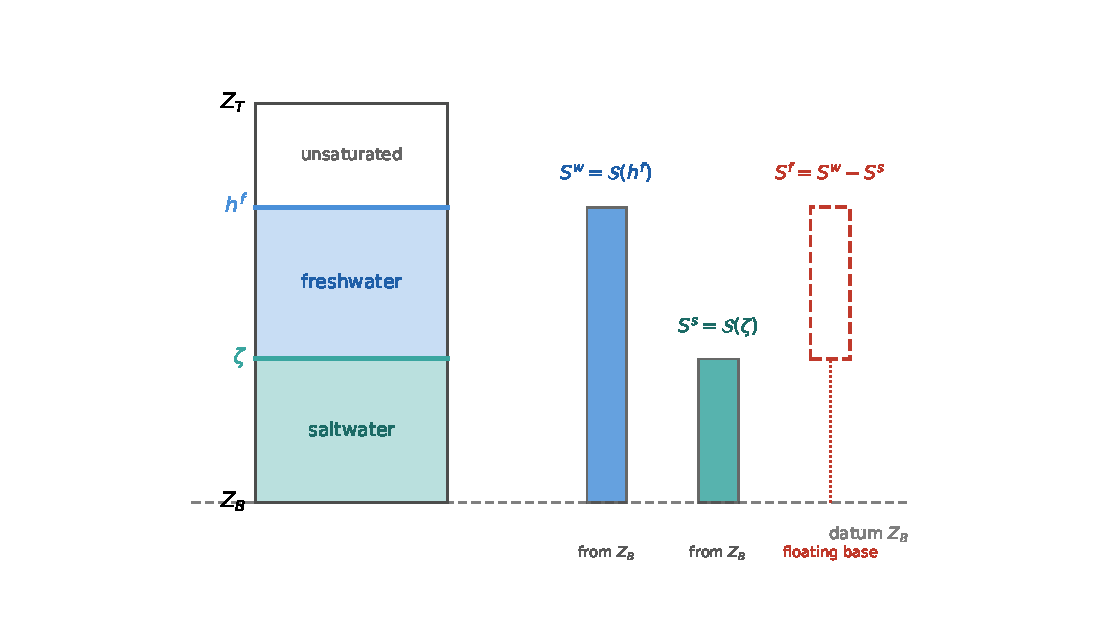
\includegraphics[width=0.86\textwidth]{./Figures/SWIInterfaceSaturations.pdf}
	\caption{Sharp-interface geometry and saturated cell fractions for one aquifer cell. The freshwater zone extends from $\zeta$ to $h^{f}$ and the saltwater zone from $Z_{B}$ to $\zeta$. The fractions $S^{w}=\mathcal{S}(h^{f})$ and $S^{s}=\mathcal{S}(\zeta)$ represent columns measured upward from $Z_{B}$ and can be evaluated with the standard MODFLOW~6 storage kernels. The freshwater fraction $S^{f}=S^{w}-S^{s}$ is bounded below by the moving interface and is therefore assembled as the difference between the two bottom-referenced columns.}
	\label{fig:swi-satbars}
\end{figure*}

\subsubsection{Smoothed saturated cell fractions and their derivatives}
\label{sec:swi-smoothsat}

The saturated cell fractions are smoothed near the cell top and bottom rather than evaluated directly from the piecewise relations in equation~\ref{eqn:swi-sats}. This is consistent with the treatment used for a standard \mf cell and keeps the saturated fraction and its head derivative continuous as the water table or interface crosses a cell boundary. SWI uses the \mf quadratic smoothing function, denoted here by $\mathcal{S}$,

\begin{equation}
\label{eqn:swi-smoothop}
\mathcal{S}(x)\equiv \mathrm{sQuadraticSaturation}(Z_{T},Z_{B},x),
\end{equation}

\noindent which is equal to the linear fraction $(x-Z_{B})/b^{\mathrm{T}}$ over most of the cell interior and transitions quadratically to $0$ near $Z_{B}$ and to $1$ near $Z_{T}$. The transition occurs over a small fraction $\Omega$ of the cell thickness. Both $\mathcal{S}$ and $\mathcal{S}'$ are continuous. The saturated cell fractions are calculated as

\begin{equation}
\label{eqn:swi-smoothsat}
S^{w}=\mathcal{S}(h^{f}),\qquad
S^{s}=\mathcal{S}(\zeta),\qquad
S^{f}=S^{w}-S^{s}.
\end{equation}

\noindent Thus, $S^{w}$ is smoothed about freshwater head and $S^{s}$ is smoothed about interface elevation; the freshwater fraction is their difference. These definitions assume the physically admissible ordering $h^{f}\ge\zeta$, which by equation~\ref{eqn:swi-gh} is equivalent to $h^{f}\ge h^{s}$; under this ordering the smoothed difference $S^{f}=S^{w}-S^{s}$ is nonnegative. From equation~\ref{eqn:swi-gh},

\begin{equation}
\label{eqn:swi-dzeta}
\frac{\partial\zeta}{\partial h^{f}}=-\alpha_{f},
\qquad
\frac{\partial\zeta}{\partial h^{s}}=\alpha_{s},
\end{equation}

\noindent and applying the chain rule to equation~\ref{eqn:swi-smoothsat} gives

\begin{equation}
\label{eqn:swi-dsat}
\frac{\partial S^{w}}{\partial h^{f}}=\mathcal{S}'(h^{f}),\quad
\frac{\partial S^{s}}{\partial h^{f}}=-\alpha_{f}\,\mathcal{S}'(\zeta),\quad
\frac{\partial S^{s}}{\partial h^{s}}=\alpha_{s}\,\mathcal{S}'(\zeta).
\end{equation}

\noindent In the cell interior, $\mathcal{S}'\to 1/b^{\mathrm{T}}$, which gives the sharp-interface slopes $b^{\mathrm{T}}\,\partial S^{s}/\partial h^{f}=-\alpha_{f}$ and $b^{\mathrm{T}}\,\partial S^{s}/\partial h^{s}=\alpha_{s}$. Near the top and bottom of a cell, the quadratic smoothing causes these derivatives to approach zero continuously. The freshwater derivatives are $\partial S^{f}/\partial h^{f}=\partial S^{w}/\partial h^{f}-\partial S^{s}/\partial h^{f}$ and $\partial S^{f}/\partial h^{s}=-\partial S^{s}/\partial h^{s}$. Because upstream weighting uses the saturated cell fraction of the upstream cell, these derivatives are nonzero only for the upstream cell.

\subsection{Finite-Volume Flow Equations}

\subsubsection{Freshwater and saltwater cell balances}

Using $S^{f}$ in place of $S^{w}$ gives the freshwater finite-volume equation

\begin{multline}
\label{eqn:swi-fvf}
A_{n}S_{n}^{f}S_{s}\,b^{\mathrm{T}}\frac{h_{n}^{f}-h_{n}^{f,t-1}}{\Delta t}
+A_{n}S_{y}\,b^{\mathrm{T}}\frac{S_{n}^{f}-S_{n}^{f,t-1}}{\Delta t}\\
=\sum_{m}\big(S_{nm}^{f,u}C_{nm}^{f}\big)\big(h_{m}^{f}-h_{n}^{f}\big)+\dot W_{f},
\end{multline}

\noindent where $A_{n}$ is horizontal cell area, $C_{nm}^{f}$ is the saturated freshwater conductance between cells $n$ and $m$, $S_{n}^{f}$ is the freshwater saturated cell fraction in cell $n$, $S_{nm}^{f,u}$ is the upstream freshwater saturated cell fraction for connection $n$--$m$, superscript $t-1$ denotes the previous time step, and $\Delta t$ is time-step length. The corresponding saltwater equation is

\begin{multline}
\label{eqn:swi-fvs}
A_{n}S_{n}^{s}S_{s}\,b^{\mathrm{T}}\frac{h_{n}^{s}-h_{n}^{s,t-1}}{\Delta t}
+A_{n}S_{y}\,b^{\mathrm{T}}\frac{S_{n}^{s}-S_{n}^{s,t-1}}{\Delta t}\\
=\sum_{m}\big(S_{nm}^{s,u}C_{nm}^{s}\big)\big(h_{m}^{s}-h_{n}^{s}\big)+\dot W_{s},
\end{multline}

\noindent where $S_{nm}^{s,u}$ is the upstream saltwater saturated cell fraction and saltwater conductance is obtained from freshwater conductance using equation~\ref{eqn:swi-Ks}, $C_{nm}^{s}=C_{nm}^{f}\,(\rho_{s}\mu_{f})/(\mu_{s}\rho_{f})$. Equations~\ref{eqn:swi-fvf} and \ref{eqn:swi-fvs} therefore have the same form, with the saturated cell fraction and conductance appropriate for each fluid.

If a fluid zone becomes very thin, $S^{f}$ or $S^{s}$ can approach zero and produce a singular or poorly conditioned matrix row. To avoid this problem, the fluid-zone conductance is not allowed to decrease below the conductance corresponding to a small minimum zone thickness. The same floor is used for both fluids and has no effect when the fluid zone has appreciable thickness.

\subsubsection{Vertical flow and the buoyancy restriction}
\label{sec:swi-vflow}

Equations~\ref{eqn:swi-fvf} and \ref{eqn:swi-fvs} apply directly to horizontal connections. Vertical connections require additional treatment because freshwater overlies saltwater within a cell. For a vertical connection between an upper and lower cell, freshwater can move between the freshwater zones and saltwater can move between the saltwater zones (fig.~\ref{fig:swi-vrestrict}). Freshwater is allowed to move upward and saltwater downward, including cases in which the two fluids move in opposite directions across the same face. Flow against buoyancy is restricted: freshwater is not allowed to move downward through saltwater, and saltwater is not allowed to move upward through freshwater. This treatment is consistent with the vertical-leakage restrictions used by \citet{huyakorn1996multiphase}.

In single-fluid mode, the interface is calculated from one continuous freshwater potential. Standard unrestricted vertical conductance is therefore used. Restricting vertical flow in this mode would disconnect cells below the interface and leave their heads underdetermined.

In two-fluid mode, vertical conductance depends on the fluid present at the shared face (at elevation $Z_{B}$ of the upper cell) and on the direction of flow. For freshwater, conductance is unrestricted when freshwater occupies the face or when flow is upward; it is reduced when saltwater occupies the face and freshwater flow is downward. For saltwater, conductance is unrestricted when saltwater occupies the face or when flow is downward; it is reduced when freshwater occupies the face and saltwater flow is upward. The interface-position and flow-direction switches are smoothed so that conductance changes continuously as the interface crosses the face. Interface-position smoothing is based on the thickness of the cell containing the interface being tested: the upper cell for freshwater and the lower cell for saltwater. A small residual conductance is retained when flow is restricted to avoid a singular row. No Newton term is applied to this vertical-conductance restriction. A smoothed-tangent Newton term was tested but did not improve convergence; nonlinear convergence is controlled primarily by interface storage.

\begin{figure*}[!ht]
	\centering
	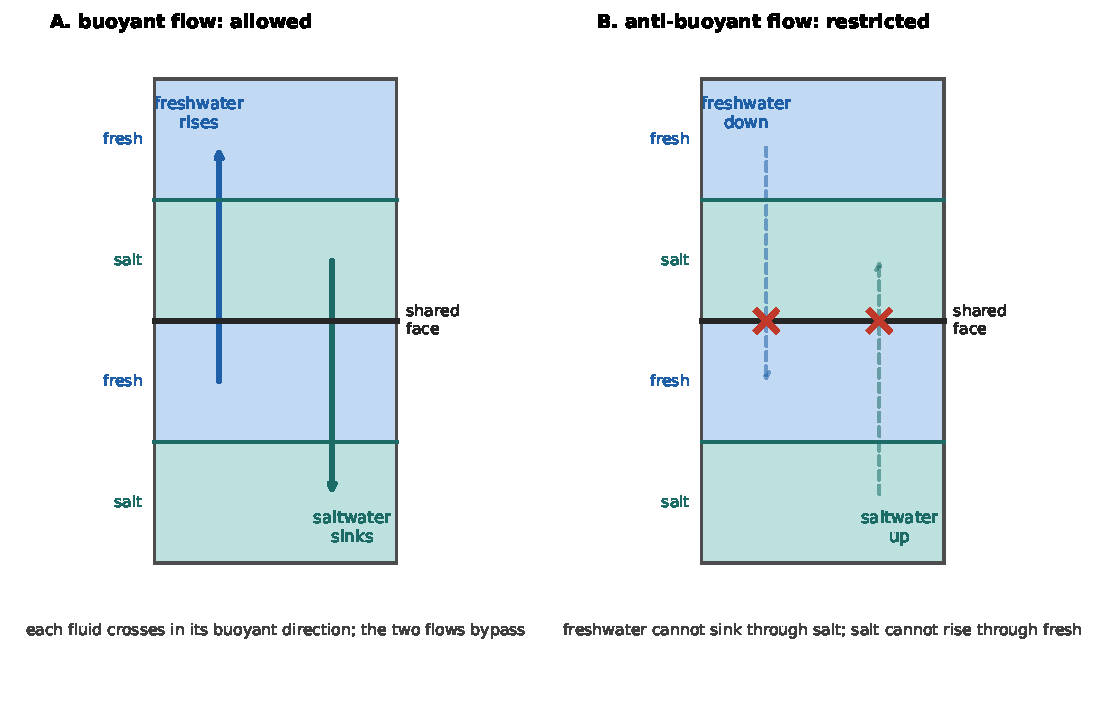
\includegraphics[width=0.74\textwidth]{./Figures/SWIVerticalRestriction.pdf}
	\caption{Vertical-flow restriction in two-fluid mode. The upper and lower cells each contain freshwater over saltwater. (A)~Buoyant flow is permitted: freshwater moves upward and saltwater moves downward across the shared face. (B)~Flow against buoyancy is restricted so that freshwater does not move downward through saltwater and saltwater does not move upward through freshwater. Interface-position and flow-direction switches are smoothed to maintain continuous conductance as the interface crosses the face.}
	\label{fig:swi-vrestrict}
\end{figure*}

\subsubsection{Relationship to the standard MODFLOW 6 assembly}
\label{sec:swi-split}

Substituting $S^{f}=S^{w}-S^{s}$ into the flow term of equation~\ref{eqn:swi-fvf} gives

\begin{multline}
\label{eqn:swi-split}
\sum_{m}\big(S^{f}C_{nm}^{f}\big)\big(h_{m}^{f}-h_{n}^{f}\big)=
\sum_{m}\big(S^{w}C_{nm}^{f}\big)\big(h_{m}^{f}-h_{n}^{f}\big)\\
-\sum_{m}\big(S^{s}C_{nm}^{f}\big)\big(h_{m}^{f}-h_{n}^{f}\big).
\end{multline}

\noindent The first term on the right is the term that would be assembled for a standard \mf model. For flow, SWI passes the combined freshwater fraction $S^{f}$ to NPF, so the flow term is assembled once using a single upstream weighting. Equation~\ref{eqn:swi-split} is therefore useful primarily for showing the relationship to the standard formulation. Storage is handled differently: the water column represented by $S^{w}$ and the saltwater column represented by $S^{s}$ are assembled separately, as described below.

\subsection{Newton--Raphson Formulation}

For the freshwater equation, define the residual as $F_{n}^{f}=Q_{n}^{f,\mathrm{sto}}-\sum_{m}Q_{nm}^{f}-\dot W_{f}=0$. A Newton expansion with respect to the two primary heads gives

\begin{multline}
\label{eqn:swi-newtf}
\Big(\tfrac{\partial F^{f}}{\partial h^{f}}\Big)^{\!k-1}\!h^{f,k}
+\Big(\tfrac{\partial F^{f}}{\partial h^{s}}\Big)^{\!k-1}\!h^{s,k}
=-F^{f,k-1}\\
+\Big(\tfrac{\partial F^{f}}{\partial h^{f}}\Big)^{\!k-1}\!h^{f,k-1}
+\Big(\tfrac{\partial F^{f}}{\partial h^{s}}\Big)^{\!k-1}\!h^{s,k-1},
\end{multline}

\noindent where $k$ is the outer-iteration index. In single-fluid mode $h^{s}$ is fixed, so terms involving $\partial/\partial h^{s}$ are omitted. In two-fluid mode, derivatives with respect to $h^{s}$ form off-diagonal blocks that are added through the SWI--SWI exchange.

\subsubsection{Flow term}

For a freshwater connection between cells $n$ and $m$, Newton linearization of the flow term gives the following matrix coefficients:

\begin{align}
\label{eqn:swi-fnflow}
h_{n}^{f,k}:&\;\;
-S^{f}C_{nm}^{f}+\frac{\partial S^{f}}{\partial h_{n}^{f}}C_{nm}^{f}\Delta h^{f},\\
h_{m}^{f,k}:&\;\;
\;\;\;S^{f}C_{nm}^{f}+\frac{\partial S^{f}}{\partial h_{m}^{f}}C_{nm}^{f}\Delta h^{f},\\
h_{n}^{s,k}:&\;\;
\frac{\partial S^{f}}{\partial h_{n}^{s}}C_{nm}^{f}\Delta h^{f},\\
h_{m}^{s,k}:&\;\;
\frac{\partial S^{f}}{\partial h_{m}^{s}}C_{nm}^{f}\Delta h^{f},
\end{align}

\noindent where $\Delta h^{f}=h_{m}^{f,k-1}-h_{n}^{f,k-1}$. Products involving heads from iteration $k-1$ are moved to the right-hand side as in equation~\ref{eqn:swi-newtf}. NPF assembles the first two terms after SWI supplies $S^{f}$ and $\partial S^{f}/\partial h^{f}$. The last two terms are cross-model contributions added by the SWI--SWI exchange. The upstream derivative used by NPF is $\partial S^{f}/\partial h^{f}=\mathcal{S}'(h^{f})+\alpha_{f}\mathcal{S}'(\zeta)$. Although the interface contribution is multiplied by $\alpha_{f}$, it enters the flow Jacobian multiplied by the intercell head difference $\Delta h^{f}$ and therefore remains a bounded correction to the conductance. The saltwater flow terms are obtained by using $S^{s}$, $C^{s}$, and the corresponding derivatives.

\subsubsection{Storage term and the bottom-referencing constraint}
\label{sec:swi-storage}

Freshwater storage cannot be assembled by simply passing $S^{f}$ to the standard \mf storage kernels. Those kernels assume that the supplied saturated fraction represents a column extending upward from the cell bottom. For the compressible term, the fluid mid-elevation is represented as $Z_{B}+\tfrac12 b^{\mathrm{T}}S$; the drainable term likewise references water volume to $Z_{B}$. These assumptions are valid for $S^{w}=\mathcal{S}(h^{f})$ and $S^{s}=\mathcal{S}(\zeta)$ because both represent columns measured upward from $Z_{B}$. They are not valid for $S^{f}=S^{w}-S^{s}$ because the freshwater zone is bounded below by $\zeta$ (figure~\ref{fig:swi-satbars}).

Direct use of $S^{f}$ also causes a numerical problem. In the unsmoothed cell interior, the drainable-storage sensitivity of freshwater thickness is

\begin{equation}
\label{eqn:swi-zonederiv}
\frac{\partial\big(b^{\mathrm{T}}S^{f}\big)}{\partial h^{f}}
=\frac{\partial\big(h^{f}-\zeta\big)}{\partial h^{f}}
=1+\alpha_{f}\approx 41,
\end{equation}

\noindent so the interface contribution to $\partial S^{f}/\partial h^{f}=\mathcal{S}'(h^{f})+\alpha_{f}\mathcal{S}'(\zeta)$ is amplified by $\alpha_{f}$, which is about 40 for the default densities. Tests showed that using $S^{f}$ directly in the standard storage assembly with this amplified tangent can produce false convergence in transient unconfined simulations. The two-column assembly described below avoids both the bottom-referencing problem and this numerical behavior:

\begin{equation}
\label{eqn:swi-twocol}
Q_{n}^{f,\mathrm{sto}}\big(S^{f}\big)
=\underbrace{Q_{n}^{\mathrm{sto}}\big(S^{w}\big)}_{\text{water column}}
-\underbrace{Q_{n}^{\mathrm{sto}}\big(S^{s}\big)}_{\text{salt column}},
\end{equation}

\noindent The first term is the standard STO assembly for the water column. The second term uses the same storage kernels for the column from $Z_{B}$ to $\zeta$. The freshwater fraction $S^{f}$ is therefore not passed directly to the storage kernels.

The two-column storage calculation is divided between the \mf Picard and Newton contributions. In the Picard (\texttt{fc}) contribution, STO assembles the water-column diagonal and right-hand side. The salt-column drainable-storage term is added using a chord slope, which avoids placing the $\alpha_{f}$-amplified interface tangent on the Picard diagonal. In the Newton (\texttt{fn}) contribution, the smoothed interface tangent $\big(V_{n}S_{y}/\Delta t\big)\alpha_{f}\mathcal{S}'(\zeta)$, where $V_{n}=A_{n}b^{\mathrm{T}}$, is added to the diagonal together with the corresponding right-hand-side term. These terms cancel at convergence and therefore alter the Jacobian without altering the converged residual. The saltwater storage terms are assembled in the same way using the appropriate saltwater derivatives.

\subsubsection{Cross-connection terms and the SWI--SWI exchange}
\label{sec:swi-cross}

In two-fluid mode, freshwater and saltwater models use coincident grids, and each freshwater cell is connected to the corresponding saltwater cell through a SWI--SWI exchange. NPF and STO assemble terms involving the primary head of each model. Cross derivatives, $\partial F^{f}/\partial h^{s}$ and $\partial F^{s}/\partial h^{f}$, are added at the exchange connection. These are Jacobian terms: each off-diagonal coefficient is accompanied by the corresponding current-head term on the right-hand side so that the contribution vanishes from the residual at convergence.

The largest cross-model contributions generally come from drainable storage. For the freshwater equation, the coefficient at the coincident freshwater--saltwater connection is

\begin{equation}
\label{eqn:swi-crossf}
\frac{V_{n}S_{y}}{\Delta t}\frac{\partial S_{n}^{f}}{\partial h_{n}^{s}}
=-\frac{V_{n}S_{y}}{\Delta t}\frac{\partial S_{n}^{s}}{\partial h_{n}^{s}},
\end{equation}

\noindent and the saltwater-equation cross coefficient, with respect to $h^{f}$, is

\begin{equation}
\label{eqn:swi-crosss}
\frac{V_{n}S_{y}}{\Delta t}\frac{\partial S_{n}^{s}}{\partial h_{n}^{f}}.
\end{equation}

\noindent Flow cross terms described above are added at the same exchange connection. The current implementation omits cross derivatives associated with compressible storage ($S_{s}$); only the drainable-storage ($S_{y}$) cross terms in equations~\ref{eqn:swi-crossf} and \ref{eqn:swi-crosss} are included. Because the cross terms cancel at convergence, this omission affects the rate of convergence but not the converged solution. As the freshwater or saltwater saturated fraction approaches zero, the corresponding fluid is naturally prevented from leaving a cell it no longer occupies, so no separate interface-thickness limiter is needed in the storage terms. The conductance floor described previously is retained only to keep the linear system nonsingular. Options are provided to disable cross-storage and cross-flow terms for development and testing; when cross-flow terms are disabled, the associated off-diagonal matrix positions are also omitted.

\subsection{Saltwater Head and Boundary Conditions}
\label{sec:swi-bc}

The SWI formulation uses freshwater head $h^{f}$ and saltwater head $h^{s}$, each referenced to a column of the corresponding fluid. At pressure $p$ and elevation $z$, $h^{f}=z+p/(\rho_{f}g)$ and $h^{s}=z+p/(\rho_{s}g)$, where $g$ is gravitational acceleration. Heads specified or simulated in the freshwater model are freshwater heads. In a two-fluid simulation, heads in the saltwater model are saltwater heads.

In single-fluid mode, $h^{s}$ is prescribed because the saltwater is static. The default value is zero. A constant value can be specified with the SALTWATER\_HEAD option, or a SALTWATER\_HEAD array can be varied by stress period using the Time-Varying Array (TVA) Utility. For a coastal application, $h^{s}$ normally represents sea level. In two-fluid mode, $h^{s}$ is simulated by the saltwater model and these inputs are not used.

For a seafloor boundary in the freshwater model, the specified head must be the equivalent freshwater head produced by the overlying seawater column. This applies, for example, to General-Head Boundary or Constant-Head cells. If sea level is $h_{\mathrm{sea}}$ and seafloor elevation is $z$, pressure at the seafloor is $\rho_{s}g(h_{\mathrm{sea}}-z)$ and the equivalent freshwater head is

\begin{equation}
\label{eqn:swi-hfeq}
h^{f}=h_{\mathrm{sea}}+\frac{\rho_{s}-\rho_{f}}{\rho_{f}}\big(h_{\mathrm{sea}}-z\big)
=h_{\mathrm{sea}}+\frac{h_{\mathrm{sea}}-z}{\alpha_{f}},
\end{equation}

\noindent For the default densities, the equivalent freshwater head exceeds sea level by 0.025 times the water depth above the seafloor. Specifying sea level directly as freshwater head would understate seafloor pressure and shift the simulated interface. Saltwater head must be prescribed consistently. With $h^{f}$ from equation~\ref{eqn:swi-hfeq} and $h^{s}=h_{\mathrm{sea}}$, equation~\ref{eqn:swi-gh} gives $\zeta=z$, so the interface intersects the seafloor at the boundary. If sea level varies with time, both the freshwater boundary heads and prescribed saltwater head must vary consistently. In the saltwater model of a two-fluid simulation, the seafloor boundary head is the saltwater head and is equal to sea level.

\subsection{Flow Reduction for Wells}
\label{sec:swi-afr}

A pumping well can remove freshwater faster than the freshwater zone can supply it. From equation~\ref{eqn:swi-gh}, a freshwater-head decline of a given magnitude raises the interface by $\alpha_{f}$ times that magnitude, so the freshwater thickness can approach zero even though the cell remains saturated. A specified withdrawal that continues after the freshwater zone has effectively disappeared can drive head to very low values and prevent nonlinear convergence. The AUTO\_FLOW\_REDUCE option of the Well (WEL) Package handles a similar problem when an ordinary model cell dewaters. With SWI, the reduction is referenced to the thickness of the fluid zone.

The \emph{flow-reduction interval} is $[Z_{R,B},\,Z_{R,T}]$. By default, $Z_{R,B}=Z_{B}$ and $Z_{R,T}=Z_{T}$, which gives the standard \mf behavior. SWI modifies this interval to match the part of the cell occupied by the simulated fluid. For freshwater, $Z_{R,B}=\max(Z_{B},\zeta)$; for saltwater, $Z_{R,T}=\min(Z_{T},\zeta)$. The reduced withdrawal rate is

\begin{equation}
\label{eqn:swi-afr}
Q_{n}^{\mathrm{wel}}=\hat Q_{n}^{\mathrm{wel}}\,
\mathrm{sQuadraticSaturation}\big(Z_{R,B}+\omega,\,Z_{R,B},\,\min(h,\,Z_{R,T})\big),
\end{equation}

\noindent where $Q_{n}^{\mathrm{wel}}$ is the reduced withdrawal rate for the well in cell $n$, $\hat Q_{n}^{\mathrm{wel}}$ is the specified withdrawal rate, $h$ is the head in the model containing the well, and $\omega$ is the reduction thickness specified with AUTO\_FLOW\_REDUCE, either as a fraction of cell thickness or, with FLOW\_REDUCTION\_LENGTH, as a length. The rate decreases smoothly to zero as the fluid thickness available to the well falls below $\omega$. In an unconfined freshwater cell, the controlling thickness is $h^{f}-\zeta$. In a confined freshwater cell, the argument is capped at $Z_{T}$ and the controlling thickness is $Z_{T}-\zeta$. In a saltwater cell, the capped argument is $\zeta$ and the controlling thickness is $\zeta-Z_{B}$. Because SWI can narrow the available fluid interval even in a confined cell, flow reduction applies to confined as well as convertible cells when that interval has been modified.

The flow-reduction interval is updated once per outer iteration from the current heads. On the first iteration of a time step it is updated directly; on subsequent iterations it moves halfway toward the current interface position. This under-relaxation reduces oscillation between pumping and shutoff when the interface controls the reduction. No Newton derivative is included for the interface-controlled part of the reduction. Where head itself controls the taper, the standard AUTO\_FLOW\_REDUCE Newton derivative is used. Within an outer iteration, the reduction interval is deliberately lagged and under-relaxed. If the interface moves by more than the reduction thickness $\omega$ during a single time step, the interval can remain offset from the current interface until the following time step.

When pumping approaches or exceeds the sustainable rate of a fluid zone, delta-bar-delta (DBD) under-relaxation should be used in the Iterative Model Solution. Because interface movement is amplified by $\alpha_{f}$ relative to freshwater-head change, undamped head updates can cause oscillation in the well reduction. With DBD under-relaxation, the withdrawal rate decreases smoothly as the available fluid zone thins.

\subsection{Solution Considerations}

Single-fluid simulations generally converge with standard iterative-solver settings. Two-fluid simulations are more difficult because the two flow equations are coupled through the strongly nonlinear interface-storage terms. Large Newton updates can move the solution into poorly conditioned regions of the nonlinear system. Backtracking is therefore recommended for two-fluid simulations. Simulations in which well withdrawals are controlled by the fluid-zone reduction described above should also use DBD under-relaxation. These solver controls affect the convergence path, not the converged equations.

SWI represents the interface with one elevation per cell and does not track the tip or toe within a cell where one fluid zone pinches out. Tip and toe locations are therefore resolved only to the grid-cell scale. This can affect more than the plotted appearance of the interface. In a comparison with the SHARP model \citep{essaid1990}, which tracks tip and toe locations within a cell, the SWI interface on the SHARP grid intersected the confining layer several cells from the SHARP location and was too shallow near the tip. Refining the grid by a factor of four reduced the interface-elevation error near the tip by about an order of magnitude and moved the tip much closer to the SHARP result. Models converted from sharp-interface codes with subcell tip and toe tracking, such as SHARP and SWI2 \citep{bakker2013documentation}, may therefore require additional refinement near pinch-out locations. Grid convergence should be evaluated where a fluid zone is expected to terminate.

\subsection{Limitations}
\label{sec:swi-limitations}

SWI replaces the default NPF and STO formulation and, in two-fluid mode, adds a second coupled flow model. Several \mf capabilities assume the standard single-fluid cell formulation and are not currently compatible with SWI. The principal limitations are listed below.

\begin{itemize}

\item \textbf{Newton formulation required.} SWI requires the \mf Newton--Raphson formulation. The interface-storage tangent is included as a Newton contribution, and the Picard-only formulation is not supported.

\item \textbf{Staggered and partially overlapping connections.} Two connection geometries are not supported. Staggered horizontal connections, in which laterally adjacent cells are vertically offset, are treated with the horizontal fluid-zone conductance, which has not been formulated for a partially overlapping face. Vertical connections are assumed to share a horizontal face at a single elevation, taken as the bottom of the upper cell; vertical connections that do not satisfy this assumption are not supported by the interface-at-face restriction.

\item \textbf{Horizontal Flow Barrier (HFB) Package.} HFB modifies intercell conductance to represent a low-permeability barrier. Its interaction with the fluid-specific conductance scaling used by SWI has not been formulated or tested.

\item \textbf{XT3D and ghost-node correction (GNC).} SWI currently uses the standard two-point conductance formulation. XT3D and GNC alter the flux stencil and are not applied to SWI flow terms.

\item \textbf{GWF--GWF coupling and local grid refinement (LGR).} Two-fluid mode uses a SWI--SWI exchange between coincident freshwater and saltwater grids. Other GWF--GWF exchanges involving an SWI model, including LGR, are not supported.

\item \textbf{Parallel simulation.} SWI flow and storage extensions and the SWI--SWI exchange are not implemented for distributed-memory parallel simulations. SWI simulations must currently be run in serial.

\item \textbf{Solute and energy transport.} SWI does not resolve concentration or temperature. Coupling an SWI flow model to Groundwater Transport (GWT) or Groundwater Energy (GWE) is not currently defined. Applications that require a resolved salinity field or other transported density-dependent constituent should use a full variable-density flow and transport approach, such as coupled MODFLOW~6 GWF and GWT models with BUY, SEAWAT, or SUTRA.

\item \textbf{Particle tracking.} The two-fluid velocity field and interface geometry calculated by SWI are not currently available to the Particle Tracking (PRT) model.

\item \textbf{Buoyancy and viscosity packages.} Density and viscosity effects are already included in SWI through $\alpha_{f}$, $\alpha_{s}$, and the saltwater conductance scaling in equation~\ref{eqn:swi-Ks}. The Buoyancy (BUY) and Viscosity (VSC) Packages are therefore not used with SWI.

\item \textbf{Advanced stress packages.} Advanced stress packages such as Multi-Aquifer Well, Streamflow Routing, Lake, and Unsaturated Zone Flow use the standard cell head and saturated-cell formulation. Their interaction with the fluid-specific SWI formulation has not been developed or tested.

\end{itemize}

\subsection{Summary}

The SWI Package provides a sharp-interface formulation for freshwater and saltwater flow in \mf. NPF flow terms use the saturated cell fraction of the simulated fluid, and saltwater conductance is adjusted for density and viscosity. In two-fluid mode, vertical flow is restricted to prevent movement against buoyancy through the opposing fluid. STO terms are assembled from bottom-referenced water and saltwater columns rather than directly from the freshwater saturated fraction, and interface-related tangent terms are included through the Newton formulation. The interface is recalculated from the current freshwater and saltwater heads during each iteration. In two-fluid simulations, cross-model derivatives are added through the SWI--SWI exchange. AUTO\_FLOW\_REDUCE is referenced to the thickness of the simulated fluid zone so that well withdrawal decreases as that zone becomes thin. Current package limitations are described in the preceding section.
